\documentclass{article}


% if you need to pass options to natbib, use, e.g.:
%     \PassOptionsToPackage{numbers, compress}{natbib}
% before loading neurips_2022


% ready for submission
% \usepackage{neurips_2022}


% to compile a preprint version, e.g., for submission to arXiv, add add the
% [preprint] option:
\usepackage[preprint]{neurips_2022}


% to compile a camera-ready version, add the [final] option, e.g.:
% \usepackage[final]{neurips_2022}


% to avoid loading the natbib package, add option nonatbib:
%    \usepackage[nonatbib]{neurips_2022}


\usepackage[utf8]{inputenc} % allow utf-8 input
\usepackage[T1]{fontenc}    % use 8-bit T1 fonts
\usepackage{hyperref}       % hyperlinks
\usepackage{url}            % simple URL typesetting
\usepackage{booktabs}       % professional-quality tables
\usepackage{amsfonts}       % blackboard math symbols
\usepackage{nicefrac}       % compact symbols for 1/2, etc.
\usepackage{microtype}      % microtypography
\usepackage{xcolor}         % colors

% my personal packages
\usepackage{tablefootnote}
\usepackage{graphicx}
\bibliographystyle{plainnat}


% \title{PPO Agent for LifeSim: a custom Gymnasium Environment based on human daily life simulation}
\title{PPO Agent for LifeSteps: a simulation based on human daily life decisions}


% The \author macro works with any number of authors. There are two commands
% used to separate the names and addresses of multiple authors: \And and \AND.
%
% Using \And between authors leaves it to LaTeX to determine where to break the
% lines. Using \AND forces a line break at that point. So, if LaTeX puts 3 of 4
% authors names on the first line, and the last on the second line, try using
% \AND instead of \And before the third author name.


\author{%
  Daniel Bernardi\\
  MSc Computer Engineering\\
  Alma Mater Studiorum - Bologna\\
  \texttt{daniel.bernardi@studio.unibo.it} \\
  \texttt{daniel\_bernardi@outlook.it}
}


\begin{document}


\maketitle

\begin{abstract}
  This paper presents an implementation of a Reinforcement Learning agent based on a Proximal Policy Optimization algorithm. The agent plays on LifeSteps, a simple custom Gymnasium Environment that simulates some basic human daily decisions (and their developments on life), also presented and developed for this paper.
\end{abstract}

\section{Background}

\subsection{Gymnasium}
Gymnasium is an API for Reinforcement Learning. It provides many environments that can be used to train and evaluate RL Algorithms, including the support support for incorporating new custom environments into the local installation. It can be useful because the custom environment, once registered in the local database of environments, will be ready to use as any of the others, garanteeing a standard usage and the possibility to use Wrappers and Utilities provided by the Gymnasium library.

\subsection{Proximal Policy Optimization}
The implementation of a Proximal Policy Optimization algorithm is one of the central parts of this project, this section will provide some background about it. Since the algorithm can be implemented in various ways, further explanations will be based on the project's implementation.

The ideas behind PPO come from Policy Gradient methods and Trust Region methods.

Policy Gradient methods are based on the computation of the policy gradient that can be used as input for a stochastic gradient ascent algorithm. To make good use of the already existing libraries that perform automatic differentiation, this gradient estimator can be obtained by differentiating an objective function with those softwares.

TRPO (Trust Region Policy Optimization, \citet{DBLP:journals/corr/SchulmanLMJA15}) introduced a constraint to the size of the policy update. Alternatively to the constraint, it's possible to insert a penalty into the objective function, but it turns out difficult, sometimes, to define the correct hyperparameters about the penalty for problems that can change over time during the learning.

PPO implements the idea of a constrained policy update of TRPO in a simple way, based on the following formulas:

\begin{displaymath}
L^{CLIP}(\theta) = \hat{\mathbb{E}}[min(r_t (\theta)\hat{A}_t, clip(r_t(\theta), 1-\epsilon, 1+\epsilon)\hat{A}_t]
\end{displaymath}

With \(r_t(\theta)\) being the ratio between the new and the old policy:
\begin{displaymath}
r_t(\theta) = \frac{\pi_\theta(a_t,s_t)}{\pi_{\theta_{old}}(a_t,s_t)}
\end{displaymath}

And \(\hat{A}_t\) being the advantage function.

The advantage function implemented in PPO is a truncated version of Generalized Advantage Estimation \citep{schulman2018highdimensional}

\begin{displaymath}
\hat{A}_t = \delta_t + (\gamma\lambda)\delta_{t+1} + \dots + \dots + (\gamma\lambda)^{T-t+1} \delta_{T-1},
\end{displaymath}
\begin{displaymath}
{where\ }\delta_t = r_t + \gamma V(s_{t+1}) - V(s_t)
\end{displaymath}

In conclusion, the objective to maximize proposed by PPO is:
\begin{displaymath}
L_t^{CLIP+VF+S}(\theta) = \hat{\mathbb{E}}_t [L_t^{CLIP}(\theta) - c_1 L_t^{VF}(\theta) +c_2S[\pi_\theta](s_t)]
\end{displaymath}

with \(L_t^{VF}(\theta)\) being the mean-squared error loss between the estimated and the target value function, \(S[\pi_\theta](s_t)\) being the entropy of the policy on a given state, and \(c_1\),\(c_2\) two coefficients (hyperparameters).

A more detailed description of the algorithm can be found on the original PPO paper. What has been written here will be discussed in the implementation section.

\section{LifeSteps}
LifeSteps is a single player game where the person (or the agent) needs to make decision about what action to take on each timestep. Each action has some sort of development into the life of the player, which has to play in a smart way to avoid losing the game. The game is considered won when the player is still alive at the end of the simulation, which endures for a given number of timesteps.

Since the environment works according to the Gymnasium API, it's characteristics will be explained based on the implementation.

There are two gamemodes for LifeSteps, one simple (the \textit{standard} mode), one more difficult (called \textit{monopoly} mode).

\subsection{The Standard gamemode}
Since the \textit{monopoly} gamemode is an extension of the \textit{standard}, all of the details written here will be true also for the next section.

The \textit{life} of the player is the main information contained in every environment's observation. It's implemented as an array of three integers in the interval \([0, 100)\). Each of these integers encode the quality of a characteristic of the player's life: it's \textit{financial resources}, it's \textit{health} and it's \textit{social connections} richness.

There is also another value, called \textit{friends}, which tells if the player has at least a true friend. This value changes nothing in this gamemode, but in the \textit{monopoly} gamemode it will be important. 

The actions that the player can perform are three: go to work, do some sport, enjoy a social occasion. 

When performing a specific action, the corresponding value of \textit{life} will receive a bonus. The difficulty of this simulation is on making the right choices. The agent must choose an action at each timestep, but that action will increase the score of just one of the three \textit{life} components. The other two components will decrease in a deterministic way. For example, doing sports for a timestep will give a \(10\) points bonus to the health value, but at the same time the money and social values will decrease of \(5\) points.

The critical values (in this gamemode) are health and money. If they reach the 0 value at one observation, the game ends and the player loses.

The \textbf{reward is given to the player only at the end of the simulation} and is calculated in this way:
\begin{displaymath}
    reward = {max\ ts} - {current\ ts} - {difficulty}
\end{displaymath}
if the player didn't reach the end of the game, otherwise the reward is:
\begin{displaymath}
    reward = max(difficulty - min(life[i]), 1), i=[0,1,2]
\end{displaymath}
with \(i\) being the index for the values about money, health and sociality, and \textit{difficulty} being an initialization parameter of the environment. \textbf{If the player wins the game, the reward is 1}.

\subsection{The Monopoly gamemode}

Just like in the popular table game Monopoly, in this gamemode sometimes the player may have to pick up a \textit{Chance card} that may affect positively or negatively the course of the game. In the environment context, the \textit{Chance card} is an event that can happen with probability \(p\), which increases at every timesteps, until the event comes up and \(p\) goes to zero again. In the occurrence of the event, a deficit on the health or money statistic of the player is applied, complicating the game. 

This possibility of encountering troubles is balanced by another game mechanic, which in the standard mode had no effects: the \textit{friends} state of the player. This information is either True or False, and it can change only in one way, from False to True, when the \textit{social} development of the player reaches 40 points. This means that if the player reaches, for example, 43 points on sociality, it will acquire a friend, which will be permanent even if the sociality score goes below 40. This is both a simplification of the game and also a method to diversify the game conditions.

The parameters that define the initial settings of the game are explained in Table~\ref{gm_start}. The difficulty is a parameter defined by the player at the creation of the environment, while the starting values are randomly sampled inside their range. Table~\ref{gm_behaviour} summarizes the gameplay behaviour based on the increment or decrease of state's values at each timestep. The increment for a given value is \(0\) only if the corrispondent action is not chosen. The trouble deficit on one of the life statistics goes from 0 to 4 if the player has a friend, 10 otherwise.


\begin{table}
  \caption{Gamemodes initial settings}
  \label{gm_start}
  \centering
  \begin{tabular}{lll}
    \toprule
    & Standard     & Monopoly                               \\
    \midrule
    difficulty              & \([0,100)\)   & \([0,100)\)   \\
    money start             & \([25,34)\)   & \([25,34)\)   \\
    health start            & \([25,34)\)   & \([25,34)\)   \\
    social start            & \([25,34)\)   & \([25,34)\)   \\
    friends start           & \(0\)         & \(0\)         \\
    trouble prob. start     &               & \(0.0\)       \\
    trouble deficit         &               & \([0,4],10\)      \\
    \bottomrule
  \end{tabular}
\end{table}

\subsection{An example of a LifeSteps simulation}

To better describe how the game works, in Figure~\ref{fig:A} there is an example of the first steps of an episode rendered in text mode.

M, H and S are the three life statistics values: money, health, sociality. The F value describes if the player has some friends. The last column tells if some trouble happened during the last step, indicading also how many points were lost. If the player loses pennies, the deficit goes to the money statistic, if the player get's hurt, the deficit goes to its health.

Let's take into consideration the second and third line. The selected action is sociality, so:
\begin{itemize}
    \item the M value decreases of 5 points (\(\Leftrightarrow 0-5)\);
    \item the H value decreases of 3 points (\(\Leftrightarrow 0-3)\);
    \item the S value increases of 9 points (\(\Leftrightarrow 10-1)\);
\end{itemize}
(0,0,10) is the increase on the state for that timestep (since sociality was selected), (-5,-3,-1) is the constant decrease of the state at each timestep.

In addition to that, the S value is now above the 40 threshold, which means that the player now has friends.


\begin{figure}
  \centering
  \fbox{\rule[-.5cm]{0cm}{0cm}
        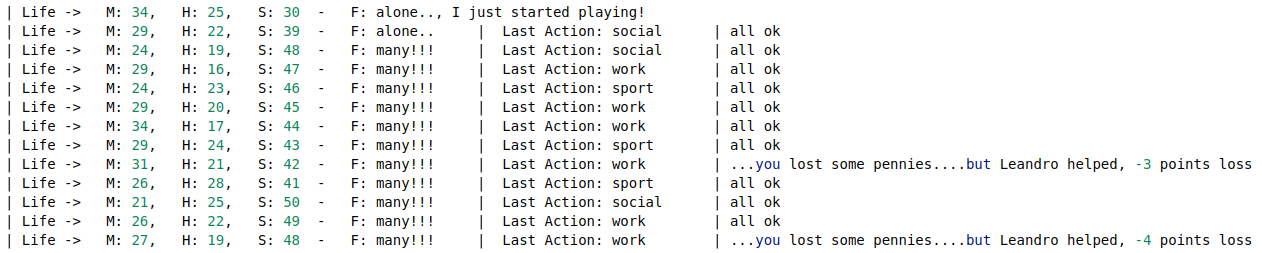
\includegraphics[width=14cm]{example_A.png}
        \rule[-.5cm]{0cm}{0cm}}
  \caption{The start of an episode in monopoly mode}
  \label{fig:A}
\end{figure}

\begin{table}
  \caption{Gamemodes increments/decrements per timestep}
  \label{gm_behaviour}
  \centering
  \begin{tabular}{llll}
    \toprule
    & Standard     & Monopoly                           \\
    \midrule
    money inc           & \(0,10\)      & \(0,10\)      \\
    health inc          & \(0,10\)      & \(0,10\)      \\
    social inc          & \(0,10\)      & \(0,10\)      \\
    money dec           & \(-5\)        & \(-5\)        \\
    health dec          & \(-3\)        & \(-3\)        \\
    social dec          & \(-1\)        & \(-1\)        \\
    trouble prob. inc   &               & \(0.03\)      \\
    \bottomrule
  \end{tabular}
\end{table}


\section{Implementation}
This section will discuss everything related to the implementation of the algorithm, the architectures of the neural networks used in the project, and the structure of the project files and Jupyter Notebook.

\subsection{Project files}
The project is programmed entirely in python and the code is subdivided in more files to semplify its understanding. The main python files are:

\begin{itemize}
    \item \textit{agent.py}: implements the PPO Agent, incapsulates the deep learning architecture, and all the methods used for training and evaluating the player inside of any gymnasium environment.
    \item \textit{memory.py}: creates the memory structures (numpy arrays) that store all the information needed for the calculation of the gradients, the advantages and the returns of each batch.
    \item \textit{utils.py}: implements some utility functions such as the calculation of advantages and returns.
\end{itemize}

The folder \textit{logs} contains (Tensorboard) logged information collected during the training of the models inside the notebook. The folder \textit{gym\_projects} contains all the file needed to register the LifeSteps environment into the local Gymnasium installation (the specific environment implementation can be found in \textit{gym\_projects/life\_sim/envs/lifesteps.py}). The folder \textit{models} contains the main checkpoints of the deep learning models.

The Jupyter Notebook with all the code about the training process is \textit{final.ipynb}.

\subsection{Notebook: final.ipynb}
Everything is implemented in Python language, using extensively the Numpy library for the management of the data, and Tensorflow to implement the deep learning models and gradients calculation.

The reproducibility of the notebook is guaranteed at the Numpy and Tensorflow levels, and all the evaluation are performed on the same environments, initialed using the same seeds. CUDA behaviour is not guaranteed to be deterministic.

The notebook is subdivided into 4 main Steps:
\begin{itemize}
    \item Step 1: training and evaluation in \textit{standard} gamemode and difficulty 40;
    \item Step 2: fine-tuning and evaluation of previous' step models in \textit{monopoly} gamemode and difficulty 40;
    \item Step 3: training and evaluation of new models in Step 2 settings;
    \item Step 4: training and evaluation of models with more units in Step 2 settings;
\end{itemize}

Further details can be found inside the notebook. The notebook was executed three times with different seeds. Each run can be seen in it's specific file called \textit{final-seed\{n\}.ipynb} with n being the seed used for the run. It's advisable to read one of those notebooks instead of the main one.

The code was executed on a laptop with an Intel® Core™ i7-8565U CPU and an Nvidia MX250 2GB GPU.


\subsection{PPO Actor-Critic}
The Actor-Critic architecture was implemented using two distinct neural networks (=> no weights sharing) with the same topology, except for the output layer. There are two hidden dense layer with 32 units each and tanh activations, and output heads with linear activations. For the Step 4 the units were increased to 128 on both models.

The original paper of PPO specifies how the algorithm should be programmed, but many variants can actually be implemented: changing the initialization of the neural networks, or the way in which the returns and advantages are calculated. The notebook follows the original PPO characteristic with some further additions.

\subsubsection{Training Loop}
Gymnasium provides the possibility to create a vector of multiple environments. This characteristic was exploited in the notebook, creating an AsyncVec (asynchronous vector) of 32 LifeStep's environments to better exploit the multiple cores during training. Even if not strictly necessary for LifeSteps, this decision speeded up the training in a considerable way, particularly in the monopoly gamemode where many epochs of training were needed to approximate a good enough policy.

PPO algorithm works by optimizing the objective for each \textbf{minibatch}, which is a portion of the total \textbf{batch} of \(timesteps * environments\) observations. The training loop iterates for a specified number of \textbf{updates}, which depends on the number of parallel environments and the maximum duration of the training (measured in timesteps). For each update, 128 actions are selected for each environment (serialized process w.r.t. the timesteps, parallelized process w.r.t. the environments), forming a batch of \(128 * 32\) sets of informations stored in Numpy NDArrays (observations, rewards, terminations, truncations, state-values). Then, the rewards are normalized and the advantages and returns are calculated for the whole batch.

The batch gets shuffled and subdivided in minibatches, for each of those we perform the optimization step for a specified number of epochs.

Some characteristic of the implementation:
\begin{itemize}
    \item The learning rate and the \(\epsilon\) are linearly annealed from the starting value to 0 at the end of the training;
    \item Orthogonal initialization of the weights in the neural network (\citep{Engstrom2020Implementation} and \citep{andrychowicz2021what} for a more specific setup);
    \item Reward scaling to the \([-1,1]\) range;
    \item Advantages normalization
\end{itemize}

The \textbf{advantages} are calculated for all the steps in the batch. The \textbf{returns} are the discounted sum of the actual rewards, with the exception of the last value, which is calculated using the state-value given by the neural network at the first observation outside the scope of the current batch.

The optimizer used is Adam, same as the original PPO paper. There was not a exhaustive search for the optimal training hyperparameters, which remain similar to the ones specified in the original paper.

\subsubsection{Loss function}
PPO is based on gradient ascent, but the popular machine learning frameworks that provides automatic differentiation are based on gradient descent methods. That's why the original PPO objective is changed and minimized for the \textbf{actor network}:

\begin{displaymath}
    Loss_{actor} = -L_t^{CLIP}(\theta) - c_2 S[\pi_\theta](s_t)
\end{displaymath}

The loss minimized on the \textbf{value network} is the mean-squared error between the returns and the approximated state-values.

\section{Results}
Tensorboard was used to log all the informations needed to analyze the 4 steps of training. Table~\ref{results} summarized the results, specifying some hyperparameters. The parameters that didn't change for all the training Steps are listed below\footnote{An exaustive search of the optimal hyperparameters was not performed and this is not an exhaustive list.}:

\begin{itemize}
    \item The max number of timesteps for each episode was 100;
    \item Difficulty is always 40;
    \item Early stopping of the training was after 6 consecutive evaluations with reward > 0;
    \item \(\gamma = 0.99\)
    \item \(\lambda = 0.95\)
    \item \(Epochs = 4\)
\end{itemize}

In the Evaluation column of Table~\ref{results} there is the value of an evaluation step performed after each of the four trainings. The evaluation is always performed on 50 episodes generated by the same 50 seeds. The number of Updates refers to the lenght of the training at the time of the early stopping\footnote{Step 2 is the only one that starts from pre-trained neural networks, so there is need to considerate also the number of updates of Step 1.}.

\begin{table}
  \caption{Training results}
  \label{results}
  \centering
  \begin{tabular}{llcrcccc}
    \toprule
    Model & GM & Units & LR & \(c_2\) & Seed & Updates & Evaluation\tablefootnote{The evaluation is the mean reward on the same 50 episodes for all the runs}\\
    \midrule
    Step 1  & std & 32  & 2.5e-4  & 0 & 14 & 350 & \textbf{1.0} \\
    & & & & & 77 & 350 & 0.92 \\
    & & & & & 39 & 350 & 1.0 \\
    \midrule
    Step 2  & mon & 32  & 1e-4   & 5e-3 & 14 & 900 & -1.14\\
    & & & & & 77 & 2343 & -2.04 \\
    & & & & & 39 & 2343 & \textbf{0.66} \\
    \midrule
    Step 3  & mon & 32  & 2.5e-4  & 5e-3 & 14 & 2300 & \textbf{0.72}\\
    & & & & & 77 & 1150 & 0.66 \\
    & & & & & 39 & 3500 & 0.40 \\
    \midrule
    Step 4  & mon & 128 & 2.5e-4  & 5e-4 & 14 & 1750 & \textbf{0.86}\\
    & & & & & 77 & 2300 & 0.86 \\
    & & & & & 39 & 1250 & -0.96 \\
    \midrule
    random-bs  
            & std & & & & 14 & & -122.3 \\
    random-bs
            & mon & & & & 14 & & -126.1 \\
    
    \bottomrule
  \end{tabular}
\end{table}

\section{Discussion}
The Deep Learning architecture solves easily the game in standard gamemode and difficulty 40 (and possibly we could even go to difficulty at 50). 

Step 2 needs some discussion. Its goal was to understand if the pre-trained networks could reduce the time of training needed to play the game in a different gamemode, similarly to what can be done in supervised learning. The results suggest that Transfer Learning in this particular case is not ideal, since the Evaluation score was good, but not excellent, and the number of update steps to obtain it was almost the same needed in Step 3. This result actually isn't that much of a surprise. Since the state is encoded into a 4 values array of integers, intuitively the features that the networks need to learn are actually very simple. On the other end, the policy must be much different because without a starting boost on the social score (to obtain a friend) the game becomes almost impossible, thanks to the Chance cards which give big deficits to the player's score.

There is not a lot to say about Step 3 and Step 4. Both the networks seem to solve the problem almost perfectly.

\subsection{A deeper analysis}
During the evaluation steps, after each training loop, for each model the data about percentages of choosen actions (on the evaluation episodes) was collected. In a very simplicistic way it describes, along with the episodes examples in the appendix, the behaviour of the agent. It can be seen that, in the monopoly gamemode, an higher selection of social actions is needed to win the game. This data is described in Table~\ref{behaviour}. 

A standard behaviour for the agent in monopoly mode is to improve the social score as first move, as seen in Figure~\ref{fig:A}.
\begin{figure}
  \centering
  \fbox{\rule[-.5cm]{0cm}{0cm}
        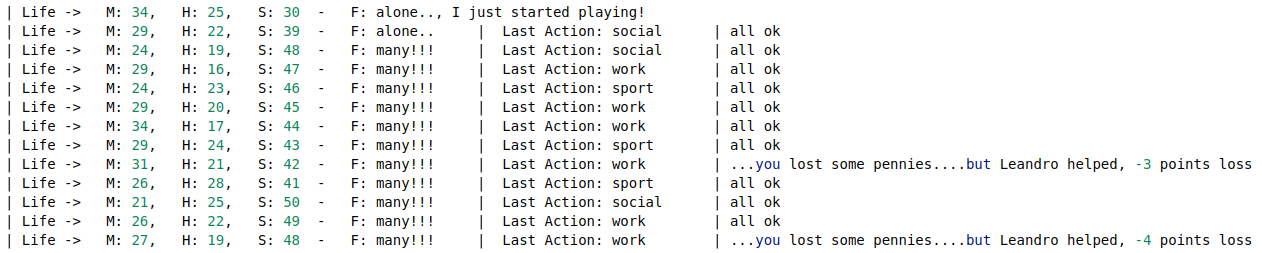
\includegraphics[width=14cm]{example_A.png}
        \rule[-.5cm]{0cm}{0cm}}
  \caption{The start of an episode in monopoly mode}
  \label{fig:A}
\end{figure}

\begin{figure}
  \centering
  \fbox{\rule[-.5cm]{0cm}{0cm}
        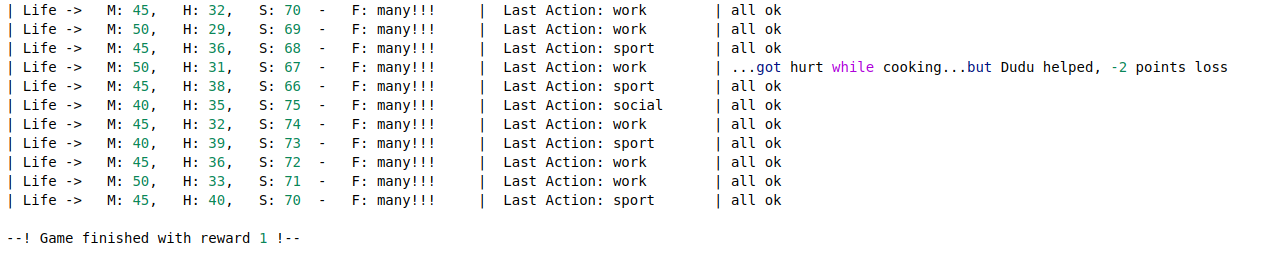
\includegraphics[width=14cm]{example_B.png}
        \rule[-.5cm]{0cm}{0cm}}
  \caption{The end of an episode in monopoly mode}
  \label{fig:B}
\end{figure} 

On the other hand, the policy does something strange at the end of a monopoly episode. As can be seen in Figure~\ref{fig:B}, the player has a very high social score. The actual social score that it needed to win the game (in that difficulty) was 30. It doesn't change much, since the presence of a friend that would reduce the score deficit of maximum 4. But anyway, the agent it's expected to behave in a more safe and robust way on higher difficulty, otherwise the final reward would go down. This lack of robustness in some case, with a policy that doesn't behave well at the end of the episodes, can be seen in Figure~\ref{fig:C}, which is an episode played by the agent trained in Step 4.

A more robust behaviour can be observed at the end of a standard episode, played by the Agent trained during Step 1. Recalling the standard gamemode rules, at difficulty 40, with 100 timesteps of episode length: the game is lost if, at the end of a fully played episode, either money or health scores are below 40; the game is lost if the episode is played for less than 100 timesteps; There are no Chance cards.\\
In Figure~\ref{fig:D} the text shows that the Agents behaviour in standard mode is more robust, since the scores are more balanced (based on the decrease-per-timestep). In fact, money would go below 40 after 5 timesteps without working, health after 5 timesteps without doing sports, and sociality after 7 timesteps without doing social actions.

\begin{figure}
  \centering
  \fbox{\rule[-.5cm]{0cm}{0cm}
        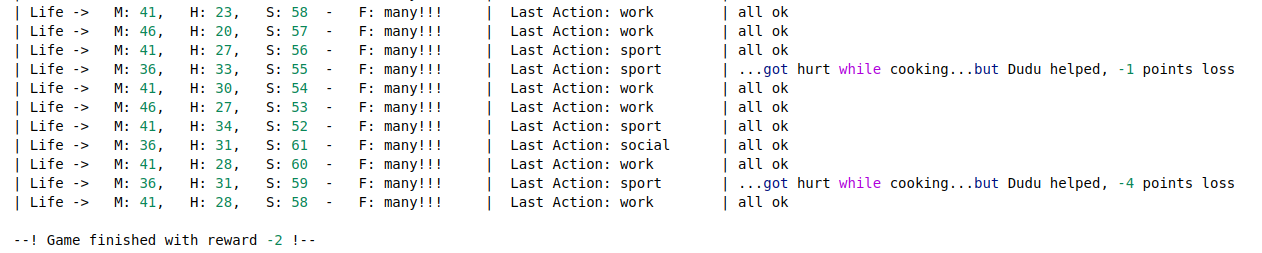
\includegraphics[width=14cm]{example_C.png}
        \rule[-.5cm]{0cm}{0cm}}
  \caption{Policy is not perfect}
  \label{fig:C}
\end{figure} 

\begin{figure}
  \centering
  \fbox{\rule[-.5cm]{0cm}{0cm}
        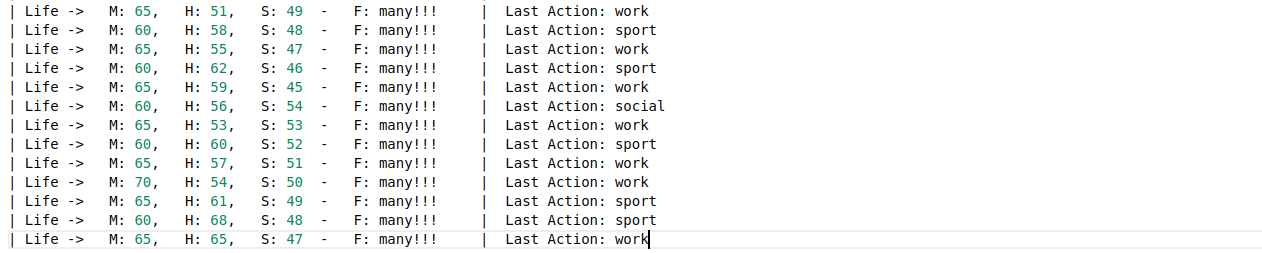
\includegraphics[width=14cm]{example_D.png}
        \rule[-.5cm]{0cm}{0cm}}
  \caption{The end of an episode in standard mode}
  \label{fig:D}
\end{figure} 

\begin{table}
  \caption{Agent's behaviour during the evaluation steps.}
  \label{behaviour}
  \centering
  \begin{tabular}{llll}
    \toprule
    & work (\%) & sport (\%) & sociality (\%)           \\
    \midrule
    Step 1  & \(54.0\)  & \(33.9\)    & \(12.1\)        \\
    Step 2  & \(52.8\)  & \(32.6\)    & \(14.6\)        \\
    Step 3  & \(53.0\)  & \(33.0\)    & \(14.0\)        \\
    Step 4  & \(53.4\)  & \(32.4\)    & \(14.2\)        \\
    \bottomrule
  \end{tabular}
\end{table}

\section{Conclusions}

\section{Useful Links and some references to useful arcticles}
\href{https://github.com/ancaah/autonomous}{Project code (github)}

\href{https://iclr-blog-track.github.io/2022/03/25/ppo-implementation-details/}{PPO implementation details}

\href{https://github.com/vwxyzjn/cleanrl/blob/master/cleanrl/ppo.py}{CleanRL PPO implementation}

\section{Submission of papers to NeurIPS 2022}


Please read the instructions below carefully and follow them faithfully.


\subsection{Style}


Papers to be submitted to NeurIPS 2022 must be prepared according to the
instructions presented here. Papers may only be up to {\bf nine} pages long,
including figures. Additional pages \emph{containing only acknowledgments and
references} are allowed. Papers that exceed the page limit will not be
reviewed, or in any other way considered for presentation at the conference.


The margins in 2022 are the same as those in 2007, which allow for $\sim$$15\%$
more words in the paper compared to earlier years.


Authors are required to use the NeurIPS \LaTeX{} style files obtainable at the
NeurIPS website as indicated below. Please make sure you use the current files
and not previous versions. Tweaking the style files may be grounds for
rejection.


\subsection{Retrieval of style files}


The style files for NeurIPS and other conference information are available on
the World Wide Web at
\begin{center}
  \url{http://www.neurips.cc/}
\end{center}
The file \verb+neurips_2022.pdf+ contains these instructions and illustrates the
various formatting requirements your NeurIPS paper must satisfy.


The only supported style file for NeurIPS 2022 is \verb+neurips_2022.sty+,
rewritten for \LaTeXe{}.  \textbf{Previous style files for \LaTeX{} 2.09,
  Microsoft Word, and RTF are no longer supported!}


The \LaTeX{} style file contains three optional arguments: \verb+final+, which
creates a camera-ready copy, \verb+preprint+, which creates a preprint for
submission to, e.g., arXiv, and \verb+nonatbib+, which will not load the
\verb+natbib+ package for you in case of package clash.


\paragraph{Preprint option}
If you wish to post a preprint of your work online, e.g., on arXiv, using the
NeurIPS style, please use the \verb+preprint+ option. This will create a
nonanonymized version of your work with the text ``Preprint. Work in progress.''
in the footer. This version may be distributed as you see fit. Please \textbf{do
  not} use the \verb+final+ option, which should \textbf{only} be used for
papers accepted to NeurIPS.


At submission time, please omit the \verb+final+ and \verb+preprint+
options. This will anonymize your submission and add line numbers to aid
review. Please do \emph{not} refer to these line numbers in your paper as they
will be removed during generation of camera-ready copies.


The file \verb+neurips_2022.tex+ may be used as a ``shell'' for writing your
paper. All you have to do is replace the author, title, abstract, and text of
the paper with your own.


The formatting instructions contained in these style files are summarized in
Sections \ref{gen_inst}, \ref{headings}, and \ref{others} below.


\section{General formatting instructions}
\label{gen_inst}


The text must be confined within a rectangle 5.5~inches (33~picas) wide and
9~inches (54~picas) long. The left margin is 1.5~inch (9~picas).  Use 10~point
type with a vertical spacing (leading) of 11~points.  Times New Roman is the
preferred typeface throughout, and will be selected for you by default.
Paragraphs are separated by \nicefrac{1}{2}~line space (5.5 points), with no
indentation.


The paper title should be 17~point, initial caps/lower case, bold, centered
between two horizontal rules. The top rule should be 4~points thick and the
bottom rule should be 1~point thick. Allow \nicefrac{1}{4}~inch space above and
below the title to rules. All pages should start at 1~inch (6~picas) from the
top of the page.


For the final version, authors' names are set in boldface, and each name is
centered above the corresponding address. The lead author's name is to be listed
first (left-most), and the co-authors' names (if different address) are set to
follow. If there is only one co-author, list both author and co-author side by
side.


Please pay special attention to the instructions in Section \ref{others}
regarding figures, tables, acknowledgments, and references.


\section{Headings: first level}
\label{headings}


All headings should be lower case (except for first word and proper nouns),
flush left, and bold.


First-level headings should be in 12-point type.


\subsection{Headings: second level}


Second-level headings should be in 10-point type.


\subsubsection{Headings: third level}


Third-level headings should be in 10-point type.


\paragraph{Paragraphs}


There is also a \verb+\paragraph+ command available, which sets the heading in
bold, flush left, and inline with the text, with the heading followed by 1\,em
of space.


\section{Citations, figures, tables, references}
\label{others}


These instructions apply to everyone.


\subsection{Citations within the text}


The \verb+natbib+ package will be loaded for you by default.  Citations may be
author/year or numeric, as long as you maintain internal consistency.  As to the
format of the references themselves, any style is acceptable as long as it is
used consistently.


The documentation for \verb+natbib+ may be found at
\begin{center}
  \url{http://mirrors.ctan.org/macros/latex/contrib/natbib/natnotes.pdf}
\end{center}
Of note is the command \verb+\citet+, which produces citations appropriate for
use in inline text.  For example,
\begin{verbatim}
   \citet{hasselmo} investigated\dots
\end{verbatim}
produces
\begin{quote}
  Hasselmo, et al.\ (1995) investigated\dots
\end{quote}


If you wish to load the \verb+natbib+ package with options, you may add the
following before loading the \verb+neurips_2022+ package:
\begin{verbatim}
   \PassOptionsToPackage{options}{natbib}
\end{verbatim}


If \verb+natbib+ clashes with another package you load, you can add the optional
argument \verb+nonatbib+ when loading the style file:
\begin{verbatim}
   \usepackage[nonatbib]{neurips_2022}
\end{verbatim}


As submission is double blind, refer to your own published work in the third
person. That is, use ``In the previous work of Jones et al.\ [4],'' not ``In our
previous work [4].'' If you cite your other papers that are not widely available
(e.g., a journal paper under review), use anonymous author names in the
citation, e.g., an author of the form ``A.\ Anonymous.''


\subsection{Footnotes}


Footnotes should be used sparingly.  If you do require a footnote, indicate
footnotes with a number\footnote{Sample of the first footnote.} in the
text. Place the footnotes at the bottom of the page on which they appear.
Precede the footnote with a horizontal rule of 2~inches (12~picas).


Note that footnotes are properly typeset \emph{after} punctuation
marks.\footnote{As in this example.}


\subsection{Figures}

All artwork must be neat, clean, and legible. Lines should be dark enough for
purposes of reproduction. The figure number and caption always appear after the
figure. Place one line space before the figure caption and one line space after
the figure. The figure caption should be lower case (except for first word and
proper nouns); figures are numbered consecutively.


You may use color figures.  However, it is best for the figure captions and the
paper body to be legible if the paper is printed in either black/white or in
color.


\subsection{Tables}


All tables must be centered, neat, clean and legible.  The table number and
title always appear before the table.  See Table~\ref{sample-table}.


Place one line space before the table title, one line space after the
table title, and one line space after the table. The table title must
be lower case (except for first word and proper nouns); tables are
numbered consecutively.


Note that publication-quality tables \emph{do not contain vertical rules.} We
strongly suggest the use of the \verb+booktabs+ package, which allows for
typesetting high-quality, professional tables:
\begin{center}
  \url{https://www.ctan.org/pkg/booktabs}
\end{center}
This package was used to typeset Table~\ref{sample-table}.


\begin{table}
  \caption{Sample table title}
  \label{sample-table}
  \centering
  \begin{tabular}{lll}
    \toprule
    \multicolumn{2}{c}{Part}                   \\
    \cmidrule(r){1-2}
    Name     & Description     & Size ($\mu$m) \\
    \midrule
    Dendrite & Input terminal  & $\sim$100     \\
    Axon     & Output terminal & $\sim$10      \\
    Soma     & Cell body       & up to $10^6$  \\
    \bottomrule
  \end{tabular}
\end{table}


\section{Final instructions}


Do not change any aspects of the formatting parameters in the style files.  In
particular, do not modify the width or length of the rectangle the text should
fit into, and do not change font sizes (except perhaps in the
\textbf{References} section; see below). Please note that pages should be
numbered.


\section{Preparing PDF files}


Please prepare submission files with paper size ``US Letter,'' and not, for
example, ``A4.''


Fonts were the main cause of problems in the past years. Your PDF file must only
contain Type 1 or Embedded TrueType fonts. Here are a few instructions to
achieve this.


\begin{itemize}


\item You should directly generate PDF files using \verb+pdflatex+.


\item You can check which fonts a PDF files uses.  In Acrobat Reader, select the
  menu Files$>$Document Properties$>$Fonts and select Show All Fonts. You can
  also use the program \verb+pdffonts+ which comes with \verb+xpdf+ and is
  available out-of-the-box on most Linux machines.


\item The IEEE has recommendations for generating PDF files whose fonts are also
  acceptable for NeurIPS. Please see
  \url{http://www.emfield.org/icuwb2010/downloads/IEEE-PDF-SpecV32.pdf}


\item \verb+xfig+ "patterned" shapes are implemented with bitmap fonts.  Use
  "solid" shapes instead.


\item The \verb+\bbold+ package almost always uses bitmap fonts.  You should use
  the equivalent AMS Fonts:
\begin{verbatim}
   \usepackage{amsfonts}
\end{verbatim}
followed by, e.g., \verb+\mathbb{R}+, \verb+\mathbb{N}+, or \verb+\mathbb{C}+
for $\mathbb{R}$, $\mathbb{N}$ or $\mathbb{C}$.  You can also use the following
workaround for reals, natural and complex:
\begin{verbatim}
   \newcommand{\RR}{I\!\!R} %real numbers
   \newcommand{\Nat}{I\!\!N} %natural numbers
   \newcommand{\CC}{I\!\!\!\!C} %complex numbers
\end{verbatim}
Note that \verb+amsfonts+ is automatically loaded by the \verb+amssymb+ package.


\end{itemize}


If your file contains type 3 fonts or non embedded TrueType fonts, we will ask
you to fix it.


\subsection{Margins in \LaTeX{}}


Most of the margin problems come from figures positioned by hand using
\verb+\special+ or other commands. We suggest using the command
\verb+\includegraphics+ from the \verb+graphicx+ package. Always specify the
figure width as a multiple of the line width as in the example below:
\begin{verbatim}
   \usepackage[pdftex]{graphicx} ...
   \includegraphics[width=0.8\linewidth]{myfile.pdf}
\end{verbatim}
See Section 4.4 in the graphics bundle documentation
(\url{http://mirrors.ctan.org/macros/latex/required/graphics/grfguide.pdf})


A number of width problems arise when \LaTeX{} cannot properly hyphenate a
line. Please give LaTeX hyphenation hints using the \verb+\-+ command when
necessary.


\begin{ack}
Use unnumbered first level headings for the acknowledgments. All acknowledgments
go at the end of the paper before the list of references. Moreover, you are required to declare
funding (financial activities supporting the submitted work) and competing interests (related financial activities outside the submitted work).
More information about this disclosure can be found at: \url{https://neurips.cc/Conferences/2022/PaperInformation/FundingDisclosure}.


Do {\bf not} include this section in the anonymized submission, only in the final paper. You can use the \texttt{ack} environment provided in the style file to autmoatically hide this section in the anonymized submission.
\end{ack}

\section*{References}


References follow the acknowledgments. Use unnumbered first-level heading for
the references. Any choice of citation style is acceptable as long as you are
consistent. It is permissible to reduce the font size to \verb+small+ (9 point)
when listing the references.
Note that the Reference section does not count towards the page limit.
\medskip


{
\small


[1] Alexander, J.A.\ \& Mozer, M.C.\ (1995) Template-based algorithms for
connectionist rule extraction. In G.\ Tesauro, D.S.\ Touretzky and T.K.\ Leen
(eds.), {\it Advances in Neural Information Processing Systems 7},
pp.\ 609--616. Cambridge, MA: MIT Press.


[2] Bower, J.M.\ \& Beeman, D.\ (1995) {\it The Book of GENESIS: Exploring
  Realistic Neural Models with the GEneral NEural SImulation System.}  New York:
TELOS/Springer--Verlag.


[3] Hasselmo, M.E., Schnell, E.\ \& Barkai, E.\ (1995) Dynamics of learning and
recall at excitatory recurrent synapses and cholinergic modulation in rat
hippocampal region CA3. {\it Journal of Neuroscience} {\bf 15}(7):5249-5262.
}


%%%%%%%%%%%%%%%%%%%%%%%%%%%%%%%%%%%%%%%%%%%%%%%%%%%%%%%%%%%%
\section*{Checklist}


%%% BEGIN INSTRUCTIONS %%%
The checklist follows the references.  Please
read the checklist guidelines carefully for information on how to answer these
questions.  For each question, change the default \answerTODO{} to \answerYes{},
\answerNo{}, or \answerNA{}.  You are strongly encouraged to include a {\bf
justification to your answer}, either by referencing the appropriate section of
your paper or providing a brief inline description.  For example:
\begin{itemize}
  \item Did you include the license to the code and datasets? \answerYes{See Section~\ref{gen_inst}.}
  \item Did you include the license to the code and datasets? \answerNo{The code and the data are proprietary.}
  \item Did you include the license to the code and datasets? \answerNA{}
\end{itemize}
Please do not modify the questions and only use the provided macros for your
answers.  Note that the Checklist section does not count towards the page
limit.  In your paper, please delete this instructions block and only keep the
Checklist section heading above along with the questions/answers below.
%%% END INSTRUCTIONS %%%


\begin{enumerate}


\item For all authors...
\begin{enumerate}
  \item Do the main claims made in the abstract and introduction accurately reflect the paper's contributions and scope?
    \answerYes{}
  \item Did you describe the limitations of your work?
    \answerTODO{}
  \item Did you discuss any potential negative societal impacts of your work?
    \answerNA{}
  \item Have you read the ethics review guidelines and ensured that your paper conforms to them?
    \answerNA{}
\end{enumerate}


\item If you are including theoretical results...
\begin{enumerate}
  \item Did you state the full set of assumptions of all theoretical results?
    \answerNA{}
        \item Did you include complete proofs of all theoretical results?
    \answerNA{}
\end{enumerate}


\item If you ran experiments...
\begin{enumerate}
  \item Did you include the code, data, and instructions needed to reproduce the main experimental results (either in the supplemental material or as a URL)?
    \answerYes{}
  \item Did you specify all the training details (e.g., data splits, hyperparameters, how they were chosen)?
    \answerYes{}
        \item Did you report error bars (e.g., with respect to the random seed after running experiments multiple times)?
    \answerNo{}
        \item Did you include the total amount of compute and the type of resources used (e.g., type of GPUs, internal cluster, or cloud provider)?
    \answerYes{}
\end{enumerate}


\item If you are using existing assets (e.g., code, data, models) or curating/releasing new assets...
\begin{enumerate}
  \item If your work uses existing assets, did you cite the creators?
    \answerNA{}
  \item Did you mention the license of the assets?
    \answerNA{}
  \item Did you include any new assets either in the supplemental material or as a URL?
    \answerNA{}
  \item Did you discuss whether and how consent was obtained from people whose data you're using/curating?
    \answerNA{}
  \item Did you discuss whether the data you are using/curating contains personally identifiable information or offensive content?
    \answerNA{}
\end{enumerate}


\item If you used crowdsourcing or conducted research with human subjects...
\begin{enumerate}
  \item Did you include the full text of instructions given to participants and screenshots, if applicable?
    \answerNA{}
  \item Did you describe any potential participant risks, with links to Institutional Review Board (IRB) approvals, if applicable?
    \answerNA{}
  \item Did you include the estimated hourly wage paid to participants and the total amount spent on participant compensation?
    \answerNA{}
\end{enumerate}


\end{enumerate}


%%%%%%%%%%%%%%%%%%%%%%%%%%%%%%%%%%%%%%%%%%%%%%%%%%%%%%%%%%%%

\bibliography{citations}

\appendix


\section{Appendix}

Example A

\begin{figure}
  \centering
  \fbox{\rule[-.5cm]{0cm}{4cm} \rule[-.5cm]{4cm}{0cm}}
  \caption{Example A.}
\end{figure}

Optionally include extra information (complete proofs, additional experiments and plots) in the appendix.
This section will often be part of the supplemental material.


\end{document}